\section{Radiation Interactions}
\subsection{General Remarks}
\subsubsection{Relationship between various classes of radiation}
\begin{itemize}
    \item Uncharged radiation: neutrons, photons
    \item Charged radiation: heavy charged particles, electrons
    \begin{itemize}
        \item Neutrons can create photons via $(n,\gamma)$
        \item Neutrons can create heavy charged particle via $(n,x)$ reactions
        \item Photons interact with electrons via EM interactions, photoelectric absorption, Compton scattering, etc.
        \item Heavy charged particles and electrons can, via EM interactions, create ionization or excitation 
    \end{itemize}
\end{itemize}
\subsubsection{Surface density / Mass thickness}
\begin{itemize}
    \item Surface density (or mass thickness)\\
    $\rho_A=\rho\times t$\\
    $[\rho_A]=g/cm^2$\\
    By using surface densities, the density dependency is removed when expressing absorber thicknesses.
    \item Atom / number density $N=\frac{\rho N_A}{A}$
    \item Electron density $N_e=\frac{\rho N_A Z}{A}$
\end{itemize}
\subsection{Interactions of Heavy Charged Particles}
\subsubsection{Energy loss behavior}
\begin{itemize}
    \item Heavy charged particles lose energy by
    \begin{itemize}
        \item Inelastic collisions with atomic electrons (most important)\\
         Due to the large ratio of projectile and electron masses, there is minimum energy loss in each interaction, and the ions travel on straight lines, slowing down continuously.
        \item Elastic scattering with nuclei
        \item Bremsstrahlung 
    \end{itemize}
    \item Heavy charged particles slow down continuously without losing intensity (compare with photon stopping).
    \item Stopping power $-\frac{dE}{dx}=S_{\text{electronic}}+S_{\text{nuclear reaction}}+S_{\text{nuclear atomic}}$
    \begin{itemize}
        \item $S_{\text{electronic}}$ is characterized by the Bethe formula (see below for full expression).
        \item $S_{\text{nuclear reaction}}$ is very small.
        \item $S_{\text{nuclear atomic}}$ is only important at the end of range (low energies).
    \end{itemize}
    See stopping power dependence in figure~\ref{fig:stopping_power_dependence}.
    \begin{figure}[ht]
        \centering
        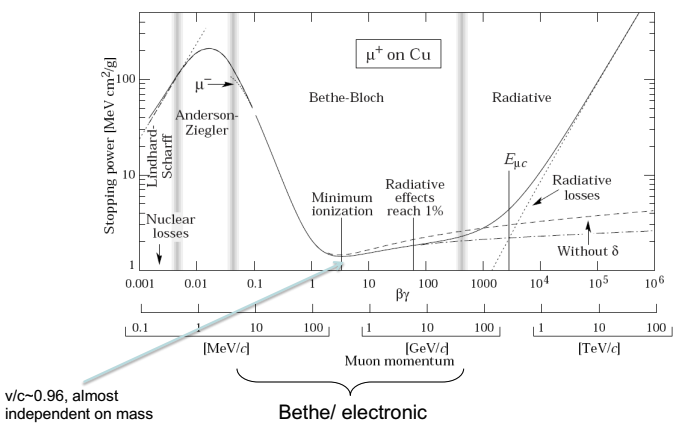
\includegraphics[width=0.8\textwidth]{images/stopping_power_dependence.png}
        \caption{Dominant factors of charged particle stopping vary with energy.}
        \label{fig:stopping_power_dependence}
    \end{figure}
    \item For compounds and mixtures, the Bragg-Kleeman rule gives\\
    $\frac{1}{N_c}\left(\frac{dE}{dx}\right)=\sum_iw_i\frac{1}{N_i}\left(\frac{d_E}{dx}\right)_i$\\
    where $N$ is the atomic number density and $w$ is the atom fraction.
    \item The Bragg curve describes how the stopping power of charged particles increase towards the end of its range, then falls off rapidly (see figure~\ref{fig:bragg_curve}). This is due to the fact that the charge of the particle is reduced by electron pickup in this region.
    \begin{figure}[ht]
        \centering
        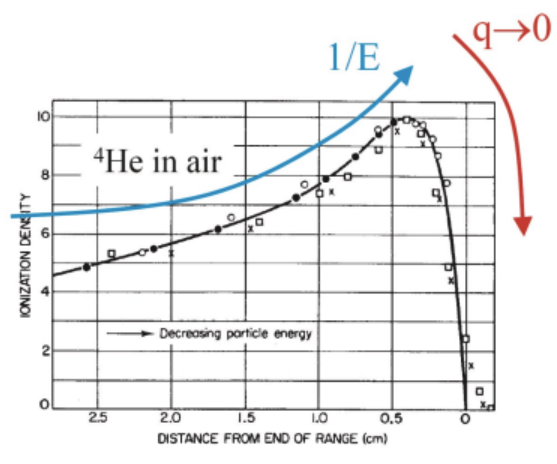
\includegraphics[width=0.5\textwidth]{images/bragg_curve.png}
        \caption{The Bragg curve.}
        \label{fig:bragg_curve}
    \end{figure}
    \item The Bragg peak, where the relative energy loss of a charged particle forms a sharp maximum at the end of its range, can be seen in figure~\ref{fig:dose_of_diff_radiation}. 
\end{itemize}

\subsubsection{Particle Identification}
\begin{itemize}
    \item The Bethe formula gives $-\frac{dE}{dx}=\frac{4\pi z^2}{m_ev^2}\left(\frac{e^2}{4\pi\varepsilon_0}\right)^2N_e\left[\ln\left(\frac{2m_ev^2}{I(1-\beta^2)}\right)-\beta^2\right]$
    \item From the Bethe formula, it is predicted that $-\frac{dE}{dx}\propto \frac{Mz^2}{E}$
    \item Therefore, by plotting $\Delta E$ vs. $E$, the particle can be identified. See figure~\ref{fig:DeltaE_E_telescope} for sample plot.
    \begin{figure}
        \centering
        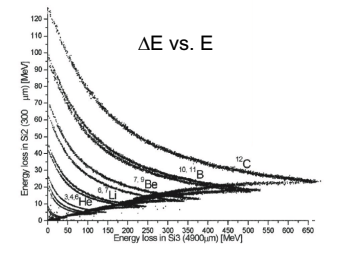
\includegraphics[width=0.55\textwidth]{images/DeltaE_E_telescope.png}
        \caption{Results of a $\Delta E-E$ Telescope.}
        \label{fig:DeltaE_E_telescope}
    \end{figure}
\end{itemize}

\subsection{Interactions of Electrons}

\subsubsection{Energy loss behavior}

\subsubsection{Range}

\subsection{Interactions of Photons}
\subsubsection{Photon attenuation}
When a photon beam passes through material, its intensity drops but the energy remains constant.\\
$I=I_0e^{-\mu x}$\\
$\mu=1/\lambda$\\
where $\mu$ is the linear attenuation coefficient, and $\lambda$ is the mean free path
\subsubsection{Four interaction processes}
\begin{enumerate}
    \item Photoelectric absorption:
    \begin{itemize}
        \item All photon energy (low energy) is transferred to a bound electron.\\
        $E_e=h\nu-E_b$ , where $E_b$ is the atomic electron binding energy
        \item $\sigma_{PE}\propto Z^{4-5}/E_\gamma^{3.5}$
    \end{itemize}
    See figure~\ref{fig:photoelectric_absorption_edges}.
    \begin{figure}[ht]
        \centering
        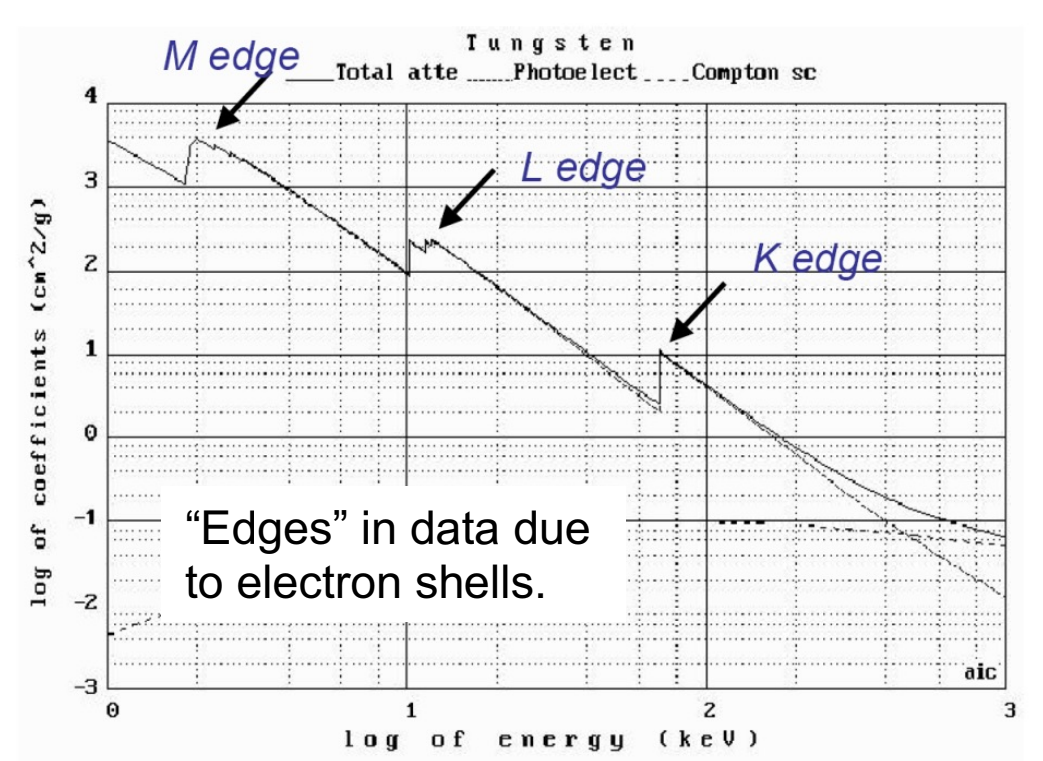
\includegraphics[width=0.5\textwidth]{images/photoelectric_absorption_edges.png}
        \caption{Photoelectric absorption behavior.}
        \label{fig:photoelectric_absorption_edges}
    \end{figure}
    \item Compton Scattering:
    \begin{itemize}
        \item Inelastic scattering of a photon with a (free) electron\\
        $E'_\gamma=E_\gamma/\left(\frac{E_\gamma}{m_ec^2}(1-\cos\theta)\right)$
        \item Largest energy transfer occurs when the scattering angle $\theta=180^\circ$ (backscattering). See figure~\ref{fig:compton_scatterint_curve}.
        \item $\sigma_{CS}\propto Z/E$\\
        The differential cross section (angular distribution) is given by the Klein-Nishina formula; the higher the photon energy, the more likely forward-scattering is.
    \end{itemize}
    \begin{figure}[ht]
        \centering
        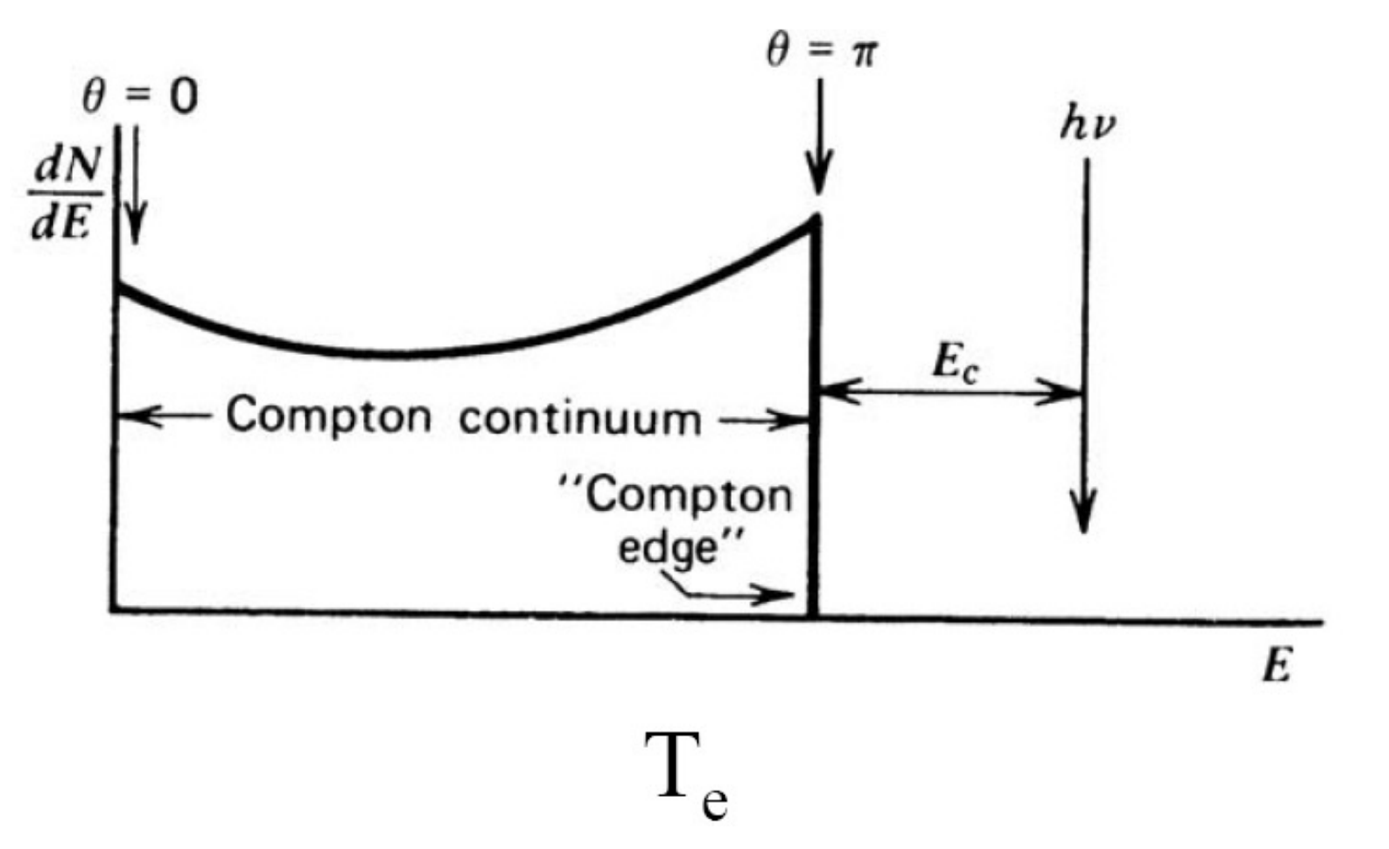
\includegraphics[width=0.5\textwidth]{images/compton_scattering.png}
        \caption{Compton scattering characteristics.}
        \label{fig:compton_scatterint_curve}
    \end{figure}
    \item Pair Production:
    \begin{itemize}
        \item When $E_\gamma>1.022\;MeV$, the photon can convert into a electron-positron pair.\\
        $E_{e^-}+E_{e^+}=E_\gamma-2m_ec^2$
        \item  After slowing down, the positron annihilates into two 511 keV photons. 
        \item $\sigma_{PP}\propto Z^2$
    \end{itemize}
    \item Coherent (Rayleigh) Scattering:\\
    Elastic scattering of light on particles smaller than the wavelength of the light.
\end{enumerate}
Which interaction process is preferred is determined by (1) Z of the matter and (2) the energy of the photon. See figure~\ref{fig:three_gamma_process}.
\begin{figure}[ht]
    \centering
    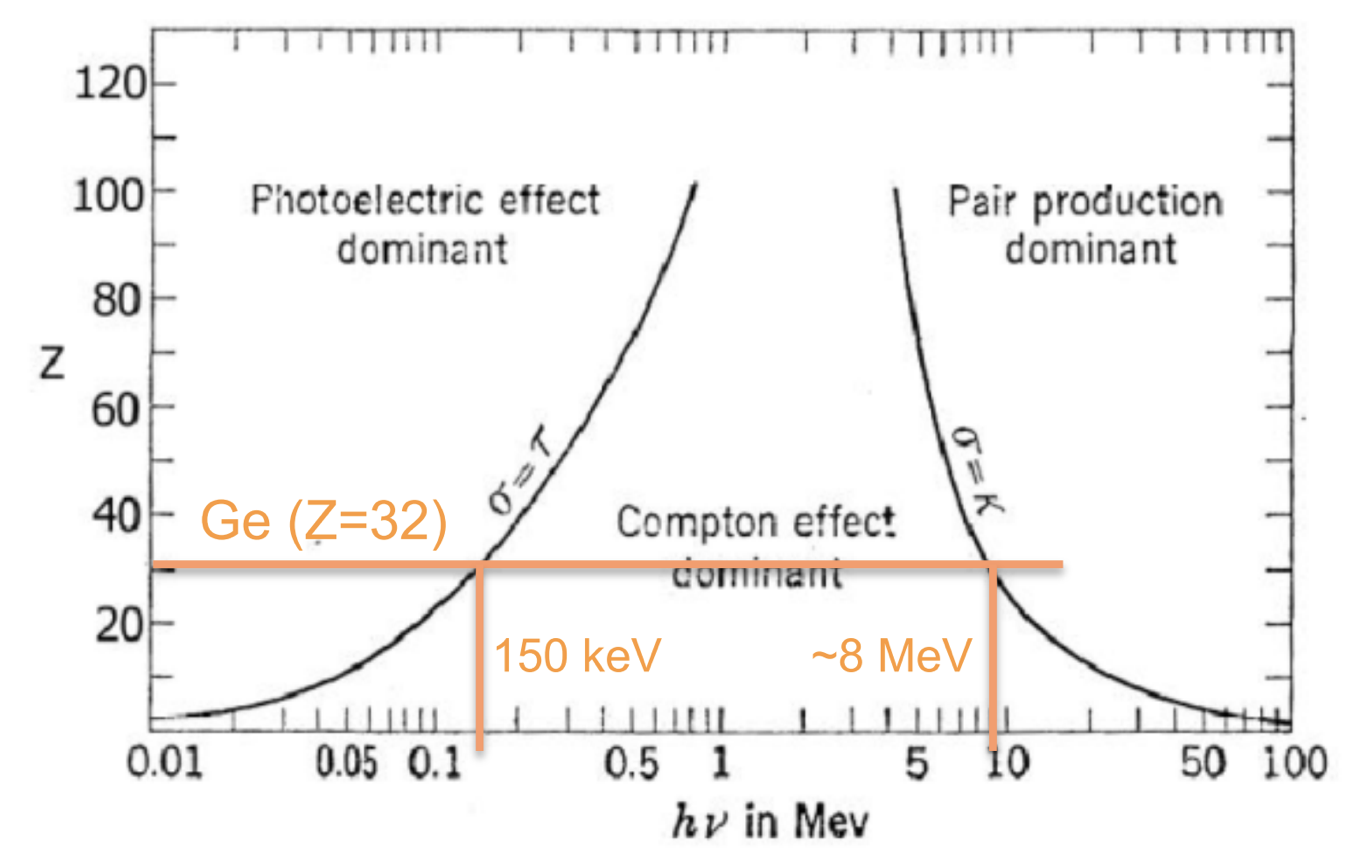
\includegraphics[width=0.6\textwidth]{images/three_gamma_process.png}
    \caption{Photon interaction process preference dependencies.}
    \label{fig:three_gamma_process}
\end{figure}
\subsection{Interactions of Neutrons}
\subsubsection{Neutron attenuation}
\begin{itemize}
    \item Neutrons are scattered by nuclei until it is of low enough energy to be absorbed. Intensity drops continuously.
    \item $I(x)=I_0e^{-\Sigma_{tot}x}$ , $\Sigma_{tot}=N\sigma_{tot}$
\end{itemize}
\subsubsection{Two classes of interactions}
\begin{enumerate}
    \item Slow neutrons (thermal \& epithermal, $<1$ keV) prefer:
    \begin{itemize}
        \item Elastic scattering
        \item Capture $(n,\gamma)$
        \item Charged particle production $(n,p),\;(n,\alpha)$ ...
        \item Fission $(n,f)$
    \end{itemize}
    \item Fast neutrons ($>1$ keV) prefer:
    \begin{itemize}
        \item Inelastic scattering
        \item The interactions mentioned for slow neutrons are possible in this region, too.
    \end{itemize}
\end{enumerate}
\subsection{Absorption and Dose Characteristics}
Figure~\ref{fig:dose_of_diff_radiation} sums up stopping and energy deposition behavior of different types of radiation. 
\begin{figure}[ht]
    \centering
    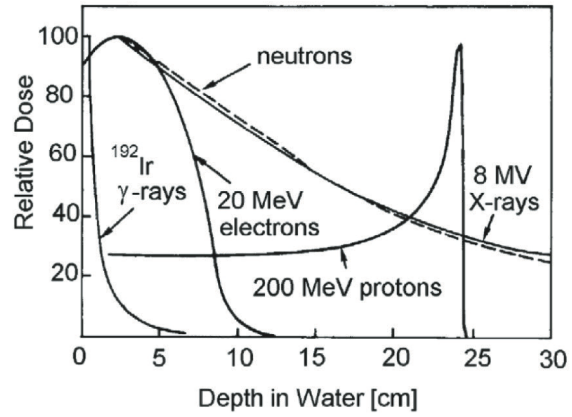
\includegraphics[width=0.5\textwidth]{images/dose_of_diff_radiation.png}
    \caption{Energy Deposition depends on radiation type.}
    \label{fig:dose_of_diff_radiation}
\end{figure}
